\section{Lokalitätsprinzip}
\textcolor{myblue}{Arbeitsbereich eines Programmes}: Die Speicherstellen welche in einem Zeitintervall $(t - \Delta t,t()$ referenziert werden.\\
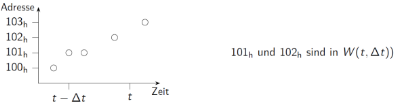
\includegraphics[width=\columnwidth]{img/lokalitaetsprinzip.png}
\textcolor{myblue}{Räumliche Lokalität}: Wenn auf eine bestimmte Adresse im Hauptspeicher zugegriffen wird ist die Wahrscheinlichkeit hoch, dass die nachfolgenden Zugriffe auf eine Adresse in der Nachbarschaft erfolgt. Im Speicher wird dies genutzt in dem man immer Datenblöcke verschiebt.\\
\textcolor{myblue}{Zeitliche Lokalität}: Wird auf eine bestimmte Adresse im Hauptspeicher zugegriffen, so ist die Wahrscheinlichkeit hoch, dass in naher Zukunft wieder darauf zugegriffen wird. Im Speichersystem will man also die zuletzt zugegriffenen Daten auf der schnellsten Stufe der Speicherhierarchie halten. \\
--> Wenn man den Arbeitsbereich kennt kann man auf den Zukünftigen schliessen.
--> Hätte man dieses Prinzip nicht, dann würde man immer nur die langsamste Speicherstufe verwenden.\\
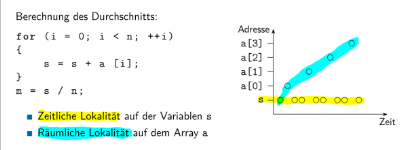
\includegraphics[width=\columnwidth]{img/lokalitaetsprinzip_beispiel.png}
